\documentclass[12pt,a4paper]{article}

\usepackage{amsmath}
\usepackage{amssymb}
\usepackage{amsthm}
\usepackage{geometry}
\usepackage{graphicx}
\usepackage{tikz}      % 用于绘制图形的主要宏包
\usepackage[utf8]{inputenc}      % UTF-8 input encoding
\usepackage[hang, small, bf]{caption} % 自定义图表标题样式

% ----- 页面布局设置 -----
\geometry{a4paper, margin=1in}

\usepackage{amsmath}
\usepackage{amssymb}

\usepackage[UTF8]{ctex}

% 设置页面边距
\geometry{a4paper, left=2.5cm, right=2.5cm, top=2.5cm, bottom=2.5cm}

% 定义定理环境
\newtheorem{law}{Law}[section]
\newtheorem{theorem}{Theorem}[section]
\theoremstyle{definition}
\newtheorem{definition}{Definition}[section]
\theoremstyle{remark}
\newtheorem*{tip}{Tip}

% 自定义向量命令
\renewcommand{\vec}[1]{\mathbf{#1}}

\title{力学原理笔记}
\author{Darryl}
\date{\today}

\begin{document}
	
	\maketitle
	
	\section{基本原理 (Elementary Principles)}
	
	\subsection{质点力学 (Mechanics of Particle)}
	
	\begin{enumerate}
		\item \textbf{半径矢量 (radius vector):} $\vec{r}$
		\item \textbf{速度矢量 (vector velocity):} $\vec{v} = \frac{d\vec{r}}{dt}$
		\item \textbf{线动量 (linear momentum):} $\vec{p} = m\vec{v}$
		\item \textbf{牛顿第二定律 (Newton's second law of motion):} $\vec{F} = \frac{d\vec{p}}{dt}$ or $\vec{F} = \frac{d}{dt}(m\vec{v}) = m\vec{a}$
		\item \textbf{加速度矢量 (vector acceleration):} $\vec{a} = \frac{d^2\vec{r}}{dt^2}$
	\end{enumerate}
	
	\begin{law}[质点线动量守恒定理]
		If the total force $\vec{F}$ is zero, then $\dot{\vec{p}} = 0$ and $\vec{p}$ is conserved.
	\end{law}
	
	\begin{enumerate}
		\setcounter{enumi}{5}
		\item \textbf{角动量 (angular momentum)} (about point O): $\vec{L} = \vec{r} \times \vec{p}$ where $\vec{r}$ is the radius vector from O to the particle.
		\item \textbf{力矩 (torque / moment of force):} $\vec{N} = \vec{r} \times \vec{F}$
	\end{enumerate}
	
	\begin{law}
		By using the vector identity $\frac{d}{dt}(\vec{A} \times \vec{B}) = \dot{\vec{A}} \times \vec{B} + \vec{A} \times \dot{\vec{B}}$, we obtain:
		\begin{align*}
			\frac{d\vec{L}}{dt} &= \frac{d}{dt}(\vec{r} \times (m\vec{v})) \\
			&= \frac{d\vec{r}}{dt} \times (m\vec{v}) + \vec{r} \times (m\frac{d\vec{v}}{dt}) \\
			&= \vec{v} \times (m\vec{v}) + \vec{r} \times (m\vec{a})
		\end{align*}
		where $\vec{v} \times \vec{v} = 0$, we obtain $\vec{N} = \frac{d\vec{L}}{dt}$.
	\end{law}
	
	\begin{law}[质点角动量守恒定理]
		If the total torque $\vec{N}$ is zero, then $\dot{\vec{L}}=0$ and $\vec{L}$ is conserved.
	\end{law}
	
	\begin{enumerate}
		\setcounter{enumi}{7}
		\item \textbf{外力做功 (work done by the external force $\vec{F}$ from point 1 to point 2):}
		\begin{equation*}
			W_{12} = \int_{1}^{2} \vec{F} \cdot d\vec{s}
		\end{equation*}
		For constant mass,
		\begin{equation*}
			\int_{1}^{2} m\frac{d\vec{v}}{dt} \cdot d\vec{s} = \int_{t_1}^{t_2} m\frac{d\vec{v}}{dt} \cdot \vec{v}dt = \int_{1}^{2} m\vec{v} \cdot d\vec{v} = \frac{1}{2}m(v_2^2 - v_1^2)
		\end{equation*}
		\item If the force field is such that work $W_{12}$ is the same for any physically possible path between points 1 and 2, the force is said to be \textbf{conservative}.
		We also obtain $\oint \vec{F} \cdot d\vec{s} = 0$ for a conservative system. By vector analysis, $W_{12}$ being independent of path $\iff \vec{F} = -\nabla V$, where $V$ is the potential energy.
	\end{enumerate}
	
	\subsection{势能 (Potential Energy: V)}
	\begin{enumerate}
		\setcounter{enumi}{9}
		\item For a conservative system:
		\begin{gather*}
			\vec{F} \cdot d\vec{s} = -dV \quad \text{or} \quad F_s = -\frac{\partial V}{\partial s} \\
			W_{12} = V_1 - V_2
		\end{gather*}
		And we have $T_1 + V_1 = T_2 + V_2$, where $T = \frac{1}{2}mv^2$ is the kinetic energy.
	\end{enumerate}
	
	\begin{law}[质点能量守恒定理]
		If the forces acting on a particle are conservative, the total energy of the particle $T+V$ is conserved.
	\end{law}
	
	
	\section{质点系力学 (Mechanics of a System of Particles)}
	
	\begin{enumerate}
		\item For the $i$-th particle of the system, the equation of motion is:
		\begin{equation*}
			\sum_{j \neq i} \vec{F}_{ji} + \vec{F}_i^{(e)} = \dot{\vec{p}}_i
		\end{equation*}
		where $\vec{F}_{ji}$ is the internal force on the $i$-th particle due to the $j$-th particle and $\vec{F}_i^{(e)}$ stands for the external force.
		
		Summed over all particles:
		\begin{equation*}
			\frac{d^2}{dt^2}\sum_i m_i \vec{r}_i = \sum_i \vec{F}_i^{(e)} + \sum_{i, j, i \neq j} \vec{F}_{ji}
		\end{equation*}
		where, according to Newton's third law ($\vec{F}_{ji} = -\vec{F}_{ij}$), the second term on the right side is zero ($\sum_{i \neq j} \vec{F}_{ji} = 0$).
		
		\item We define a vector $\vec{R}$ as the average of the radii vectors of the particles (\textbf{or, the center of mass}):
		\begin{equation*}
			\vec{R} = \frac{\sum m_i \vec{r}_i}{\sum m_i}
		\end{equation*}
		Using the definition, we obtain: $M\frac{d^2\vec{R}}{dt^2} = \vec{F}^{(e)}$, where $M = \sum m_i$ is the total mass and $\vec{F}^{(e)} = \sum_i \vec{F}_i^{(e)}$ is the total external force.
		
		\item The total linear momentum of the system:
		\begin{equation*}
			\vec{P} = \sum_i \vec{p}_i = \sum_i m_i \frac{d\vec{r}_i}{dt} = M\frac{d\vec{R}}{dt}
		\end{equation*}
	\end{enumerate}
	
	\begin{law}[质点系线动量守恒]
		If the total external force is zero, the total linear momentum is zero.
	\end{law}
	
	\begin{enumerate}
		\setcounter{enumi}{3}
		\item The total angular momentum: $\vec{L} = \sum_i \vec{r}_i \times \vec{p}_i$.
		Using this, we have:
		\begin{align*}
			\frac{d\vec{L}}{dt} &= \sum_i (\dot{\vec{r}}_i \times \vec{p}_i + \vec{r}_i \times \dot{\vec{p}}_i) \\
			&= \sum_i (\vec{v}_i \times m_i\vec{v}_i) + \sum_i \vec{r}_i \times (\vec{F}_i^{(e)} + \sum_{j \neq i} \vec{F}_{ji}) \\
			&= \sum_i \vec{r}_i \times \vec{F}_i^{(e)} + \sum_{i,j, i \neq j} \vec{r}_i \times \vec{F}_{ji}
		\end{align*}
		where the last term can be written as $\frac{1}{2}\sum_{i,j, i \neq j} (\vec{r}_i - \vec{r}_j) \times \vec{F}_{ji}$. If we assume the strong law of action and reaction ($\vec{F}_{ji}$ is parallel to $\vec{r}_i - \vec{r}_j$), this term is zero.
		Thus: $\frac{d\vec{L}}{dt} = \vec{N}^{(e)}$, where $\vec{N}^{(e)} = \sum_i \vec{r}_i \times \vec{F}_i^{(e)}$ is the total external torque.
		
	\end{enumerate}
	
	\begin{law}[质点系角动量守恒]
		For a system, $\vec{L}$ is constant in time if the external torque is zero.
	\end{law}
	
	\begin{enumerate}
		\setcounter{enumi}{4}
		\item Let $\vec{R}$ be the radius vector from O to the center of mass and let $\vec{r}'_i$ be the radius vector from the center of mass to the $i$-th particle. Then we have:
		\begin{figure}[h!]
			% 将图形居中显示
			\centering
			
			% 开始 TikZ 图形绘制环境
			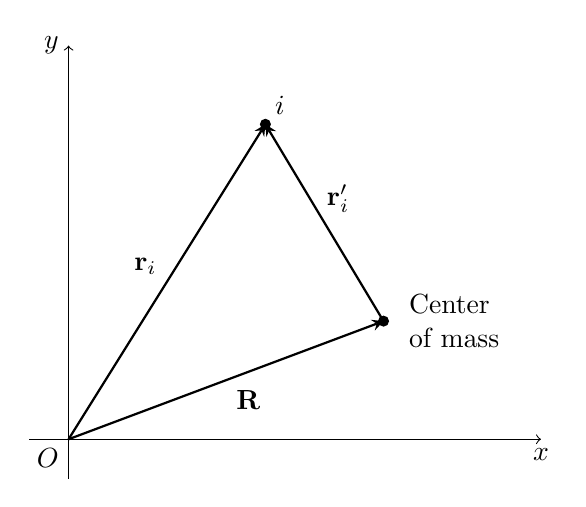
\begin{tikzpicture}[
				% 为图形中的所有箭头设置统一样式
				vector/.style={->, thick, >=stealth}
				]
				
				% ----- 1. 绘制坐标轴 -----
				% 绘制 x 轴
				\draw[->] (-0.5, 0) -- (6, 0) node[below] {$x$};
				% 绘制 y 轴
				\draw[->] (0, -0.5) -- (0, 5) node[left] {$y$};
				
				% ----- 2. 定义关键点坐标 -----
				% O: 原点
				\coordinate (O) at (0, 0);
				% i: 粒子 i 的位置
				\coordinate (I) at (2.5, 4);
				% CM: 质心 (Center of Mass) 的位置
				\coordinate (CM) at (4, 1.5);
				
				% ----- 3. 绘制矢量箭头 -----
				% 绘制从 O 到 i 的矢量 r_i
				\draw[vector] (O) -- (I) node[midway, left,yshift=2mm] {$\mathbf{r}_i$};
				
				% 绘制从 O 到 CM 的矢量 R
				\draw[vector] (O) -- (CM) node[midway, below right] {$\mathbf{R}$};
				
				% 绘制从 CM 到 i 的矢量 r'_i
				\draw[vector] (CM) -- (I) node[midway, above right,xshift=-1mm] {$\mathbf{r}'_i$};
				
				% ----- 4. 添加点和标签 -----
				% 标记原点 O
				\node[below left] at (O) {$O$};
				
				% 标记粒子点 i
				\fill (I) circle (2pt); % 在点 i 处画一个实心圆
				\node[above right] at (I) {$i$};
				
				% 标记质心点
				\fill (CM) circle (2pt); % 在质心处画一个实心圆
				\node[right, align=left, xshift=2mm] at (CM) {Center \\ of mass};
				
			\end{tikzpicture} % 结束 TikZ 环境
			
			% ----- 5. 添加图形的标题和标签 -----
			% \caption* 会生成一个没有 "Figure X:" 前缀的标题
			% 如果需要带编号的标题,请使用 \caption{...}
			\caption{The vectors involved in the shift of reference point for the angular momentum.}
			% \label 用于在文章其他地方交叉引用,例如 \ref{fig:vector_shift}
			\label{fig:vector_shift}
			
		\end{figure} % 结束 figure 环境
		\begin{equation*}
			\vec{r}_i = \vec{R} + \vec{r}'_i \implies \vec{v}_i = \vec{V} + \vec{v}'_i
		\end{equation*}
		where $\vec{V} = \frac{d\vec{R}}{dt}$ is the velocity of the center of mass and $\vec{v}'_i = \frac{d\vec{r}'_i}{dt}$ is the velocity of the $i$-th particle relative to the center of mass.
		The total angular momentum $\vec{L}$ is:
		\begin{align*}
			\vec{L} &= \sum_i m_i \vec{r}_i \times \vec{v}_i \\
			&= \sum_i m_i (\vec{R} + \vec{r}'_i) \times (\vec{V} + \vec{v}'_i) \\
			&= \sum_i m_i (\vec{R} \times \vec{V} + \vec{R} \times \vec{v}'_i + \vec{r}'_i \times \vec{V} + \vec{r}'_i \times \vec{v}'_i) \\
			&= (\sum_i m_i) \vec{R} \times \vec{V} + \vec{R} \times \frac{d}{dt}(\sum_i m_i\vec{r}'_i) + (\sum_i m_i\vec{r}'_i) \times \vec{V} + \sum_i m_i \vec{r}'_i \times \vec{v}'_i
		\end{align*}
		Since $\sum_i m_i \vec{r}'_i$ is the position vector of the center of mass relative to itself, it is zero.
		Thus, $\vec{L} = \vec{R} \times M\vec{V} + \sum_i \vec{r}'_i \times \vec{p}'_i$.
		This shows the total angular momentum is the sum of the angular momentum of the center of mass plus the angular momentum of motion about the center of mass.
		
		\item \textbf{能量方程 (Energy equation):} The total work done is
		\begin{align*}
			W_{12} &= \sum_i \int_1^2 \vec{F}_i \cdot d\vec{s}_i = \sum_i \int m_i \dot{\vec{v}}_i \cdot \vec{v}_i dt \\
			&= \sum_i \int d(\frac{1}{2} m_i v_i^2) = T_2 - T_1
		\end{align*}
		where $T = \frac{1}{2}\sum_i m_i v_i^2$ is the total kinetic energy. Using $\vec{v}_i = \vec{V} + \vec{v}'_i$:
		\begin{align*}
			T &= \frac{1}{2}\sum_i m_i (\vec{V} + \vec{v}'_i)^2 \\
			&= \frac{1}{2}\sum_i m_i (V^2 + 2\vec{V}\cdot\vec{v}'_i + {v'_i}^2) \\
			&= \frac{1}{2}(\sum_i m_i)V^2 + \vec{V}\cdot\frac{d}{dt}(\sum_i m_i\vec{r}'_i) + \frac{1}{2}\sum_i m_i {v'_i}^2
		\end{align*}
		where the last term (middle term in the expansion) is zero. Thus:
		\begin{equation*}
			T = \frac{1}{2}MV^2 + \frac{1}{2}\sum_i m_i {v'_i}^2
		\end{equation*}
		
		\item \textbf{保守系统 (For a conservative system):}
		The total work done is
		\begin{equation*}
			\sum_i \int \vec{F}_i \cdot d\vec{s}_i = -\sum_i V_i \Big|_1^2
		\end{equation*}
		When all the forces are conservative, for a pair, the total work from the internal forces is:
		\begin{equation*}
			-\int (\nabla_i V_{ij} \cdot d\vec{s}_i + \nabla_j V_{ij} \cdot d\vec{s}_j)
		\end{equation*}
		where $\nabla_i V_{ij} = -\nabla_j V_{ij}$. Note: The original notes seem to have a typo here.
		Hence, for the $ij$ pair:
		\begin{equation*}
			dW_{ij} = -(\nabla_i V_{ij} \cdot d\vec{s}_i + \nabla_j V_{ij} \cdot d\vec{s}_j) = -\nabla_i V_{ij} \cdot (d\vec{s}_i - d\vec{s}_j) = -\nabla_i V_{ij} \cdot d\vec{r}_{ij}
		\end{equation*}
		The total work for internal forces: $-\frac{1}{2} \sum_{i \neq j} \int \nabla_{ij} V_{ij} \cdot d\vec{r}_{ij} = -\frac{1}{2}\sum_{i \neq j} V_{ij} \Big|_1^2$. The factor $\frac{1}{2}$ is because in summing over both $i$ and $j$, each pair is included twice.
		
		Therefore, the total potential energy is:
		\begin{equation*}
			V = \sum_i V_i^{(e)} + \frac{1}{2} \sum_{i \neq j} V_{ij}
		\end{equation*}
		where the second term is called the \textbf{internal potential energy} of the system.
	\end{enumerate}
	
	\begin{tip}
		Assuming the potential energy between $i$-th and $j$-th particles is $V_{ij}(|\vec{r}_i - \vec{r}_j|)$ which is only dependent on relative position, its gradient satisfies that
		\begin{equation*}
			\nabla_i V_{ij}(|\vec{r}_i - \vec{r}_j|) = - \nabla_j V_{ij}(|\vec{r}_i - \vec{r}_j|)
		\end{equation*}
		or
		\begin{equation*}
			\vec{F}_{ij} = -\nabla_i V_{ij} = \nabla_j V_{ij} = -\vec{F}_{ji} \implies \text{the two forces are equal and opposite.}
		\end{equation*}
	\end{tip}
	
	\newpage
	\section{拉格朗日力学 (Lagrangian Mechanics)}
	
	\subsection{约束 (Constraints)}
	\begin{enumerate}
		\item If equations connecting the coordinates of the particles have the form $f(\vec{r}_1, \vec{r}_2, \dots, t) = 0$, they are called \textbf{holonomic}.
		For example: for a rigid body, $(\vec{r}_i - \vec{r}_j)^2 - c_{ij}^2 = 0$.
		Otherwise, they are called \textbf{non-holonomic}.
		
		\item For holonomic systems, we introduce the \textbf{generalized coordinates} to solve the problem that the equations of motion are not all independent.
		In terms of Cartesian coordinates, a system of $N$ particles free from constraints has $3N$ degrees of freedom. If there exist $k$ holonomic constraints expressed in $k$ equations, the degrees of freedom become $3N-k$.
		To eliminate the dependent coordinates, we introduce $3N-k$ independent variables $q_1, q_2, \dots, q_{3N-k}$ in terms of which $\vec{r}_i$ are expressed as:
		\begin{align*}
			\vec{r}_1 &= \vec{r}_1(q_1, q_2, \dots, q_{3N-k}, t) \\
			&\vdots \\
			\vec{r}_N &= \vec{r}_N(q_1, q_2, \dots, q_{3N-k}, t)
		\end{align*}
		By using these equations and $k$ equations of constraints we can obtain any $q_j$ as a function of $\vec{r}_i$ and $t$.
	\end{enumerate}
	
	\subsection{达朗贝尔原理和拉格朗日方程 (D'Alembert's Principle and Lagrange's Equations)}
	
	\begin{enumerate}
		\item A \textbf{virtual displacement} $\delta\vec{r}_i$ of a system is an infinitesimal change in the configuration of the system as a result of any arbitrary infinitesimal change of the coordinates $\delta q_j$, which is consistent with the forces and constraints at the given instant $t$. Suppose the system is in equilibrium, the total force $\vec{F}_i = 0$, then the virtual work:
		\begin{equation*}
			\sum_i \vec{F}_i \cdot \delta\vec{r}_i = 0
		\end{equation*}
		Decompose $\vec{F}_i = \vec{F}_i^{(a)} + \vec{f}_i$ where $\vec{F}_i^{(a)}$ is the applied force and $\vec{f}_i$ is the force of constraint.
		So that $\sum_i \vec{F}_i^{(a)} \cdot \delta\vec{r}_i + \sum_i \vec{f}_i \cdot \delta\vec{r}_i = 0$.
		We now only consider systems where the net virtual work of the forces of constraints is zero, like rigid bodies.
		Therefore, we have as the condition for equilibrium of a system: $\sum_i \vec{F}_i^{(a)} \cdot \delta\vec{r}_i = 0$, the \textbf{principle of virtual work}.
		
		\item We already have $\vec{F}_i = \dot{\vec{p}}_i$ or $\vec{F}_i - \dot{\vec{p}}_i = 0$.
		$\implies \sum_i (\vec{F}_i - \dot{\vec{p}}_i) \cdot \delta\vec{r}_i = 0$
		$\implies \sum_i (\vec{F}_i^{(a)} - \dot{\vec{p}}_i) \cdot \delta\vec{r}_i = 0$. This is \textbf{D'Alembert's principle}.
		We must now transform it into an expression of generalized coordinates, so that $\delta q_j$ can be equal to zero.
		\begin{gather*}
			\vec{r}_i = \vec{r}_i(q_1, \dots, q_n, t) \\
			\vec{v}_i = \sum_k \frac{\partial \vec{r}_i}{\partial q_k}\dot{q}_k + \frac{\partial \vec{r}_i}{\partial t} \\
			\delta\vec{r}_i = \sum_j \frac{\partial \vec{r}_i}{\partial q_j} \delta q_j \quad (\delta t = 0)
		\end{gather*}
		
		\item In terms of the generalized coordinates, the virtual work is
		\begin{equation*}
			\sum_i \vec{F}_i \cdot \delta\vec{r}_i = \sum_j \left( \sum_i \vec{F}_i \cdot \frac{\partial \vec{r}_i}{\partial q_j} \right) \delta q_j = \sum_j Q_j \delta q_j
		\end{equation*}
		where $Q_j$ are components of the generalized force, defined as $Q_j = \sum_i \vec{F}_i \cdot \frac{\partial \vec{r}_i}{\partial q_j}$.
		
		\item For the term $\sum_i \dot{\vec{p}}_i \cdot \delta\vec{r}_i = \sum_i m_i \ddot{\vec{r}}_i \cdot \delta\vec{r}_i = \sum_j \left( \sum_i m_i \ddot{\vec{r}}_i \cdot \frac{\partial \vec{r}_i}{\partial q_j} \right) \delta q_j$.
		Consider the relation:
		\begin{equation*}
			\sum_i m_i \ddot{\vec{r}}_i \cdot \frac{\partial \vec{r}_i}{\partial q_j} = \sum_i \left[ \frac{d}{dt} \left( m_i \dot{\vec{r}}_i \cdot \frac{\partial \vec{r}_i}{\partial q_j} \right) - m_i \dot{\vec{r}}_i \cdot \frac{d}{dt} \left( \frac{\partial \vec{r}_i}{\partial q_j} \right) \right]
		\end{equation*}
		Where $\frac{d}{dt}(\frac{\partial \vec{r}_i}{\partial q_j}) = \sum_k \frac{\partial^2 \vec{r}_i}{\partial q_j \partial q_k}\dot{q}_k + \frac{\partial^2 \vec{r}_i}{\partial q_j \partial t} = \frac{\partial \vec{v}_i}{\partial q_j}$.
		\begin{tip}
			$\vec{v}_i = \sum_k \frac{\partial \vec{r}_i}{\partial q_k}\dot{q}_k + \frac{\partial \vec{r}_i}{\partial t} \implies \frac{\partial \vec{v}_i}{\partial \dot{q}_j} = \frac{\partial \vec{r}_i}{\partial q_j}$
		\end{tip}
		It leads to that $\sum_i m_i \dot{\vec{r}}_i \cdot \frac{\partial \vec{v}_i}{\partial q_j} = \sum_i \frac{1}{2} \frac{\partial}{\partial q_j}(m_i v_i^2) = \frac{\partial T}{\partial q_j}$.
		And $\sum_i m_i \dot{\vec{r}}_i \cdot \frac{\partial \vec{r}_i}{\partial q_j} = \sum_i m_i \vec{v}_i \cdot \frac{\partial \vec{v}_i}{\partial \dot{q}_j} = \frac{\partial T}{\partial \dot{q}_j}$.
		Now we obtain from D'Alembert's principle $\sum_j \left[ \frac{d}{dt}\left(\frac{\partial T}{\partial \dot{q}_j}\right) - \frac{\partial T}{\partial q_j} - Q_j \right] \delta q_j = 0$.
		Since $\delta q_j$ must be independent of each other, this means that:
		\begin{equation*}
			\frac{d}{dt}\left(\frac{\partial T}{\partial \dot{q}_j}\right) - \frac{\partial T}{\partial q_j} = Q_j
		\end{equation*}
		
		\item If the whole system is conservative, then $\vec{F}_i = -\nabla_i V$.
		Then the generalized forces can be written as:
		\begin{equation*}
			Q_j = \sum_i \vec{F}_i \cdot \frac{\partial \vec{r}_i}{\partial q_j} = -\sum_i \nabla_i V \cdot \frac{\partial \vec{r}_i}{\partial q_j}
		\end{equation*}
		(T.P.) $V=V(\vec{r}_1, \dots, \vec{r}_N, t)$
		\begin{equation*}
			\implies \frac{\partial V}{\partial q_j} = \sum_i \nabla_i V \cdot \frac{\partial \vec{r}_i}{\partial q_j}
		\end{equation*}
		Therefore, $Q_j = -\frac{\partial V}{\partial q_j}$.
		
		\item Finally, we obtain:
		\begin{equation*}
			\frac{d}{dt}\left(\frac{\partial T}{\partial \dot{q}_j}\right) - \frac{\partial T}{\partial q_j} = -\frac{\partial V}{\partial q_j}
		\end{equation*}
		\begin{equation*}
			\frac{d}{dt}\left(\frac{\partial T}{\partial \dot{q}_j}\right) - \frac{\partial (T-V)}{\partial q_j} = 0
		\end{equation*}
		Also, V is independent of $\dot{q}_j$, so $\frac{\partial V}{\partial \dot{q}_j} = 0$.
		\begin{equation*}
			\frac{d}{dt}\left(\frac{\partial (T-V)}{\partial \dot{q}_j}\right) - \frac{\partial (T-V)}{\partial q_j} = 0
		\end{equation*}
		So we define the \textbf{Lagrangian} $L=T-V$, and we obtain \textbf{Lagrange's equations}:
		\begin{equation*}
			\frac{d}{dt}\left(\frac{\partial L}{\partial \dot{q}_j}\right) - \frac{\partial L}{\partial q_j} = 0
		\end{equation*}
	\end{enumerate}
	\section{Derivation of Lagrange's Equations }
	Consider a virtual displacement $\delta\vec{r}_i$ (an arbitrary infinitesimal displacement of position that could occur in the system without the passage of time).
	From D'Alembert's principle:
	\begin{equation*}
		\sum_i (\vec{F}_i - \dot{\vec{p}}_i) \cdot \delta\vec{r}_i = 0
	\end{equation*}
	where $\vec{F}_i = \vec{F}_i^{(a)} + \vec{f}_i$ ($\vec{F}_i^{(a)}$ is the applied force, $\vec{f}_i$ is the force of constraint).
	Assuming the constraint forces do no work, i.e.,
	$$ \sum_i \vec{f}_i \cdot \delta\vec{r}_i = 0. $$
	Thus, the principle becomes
	$$ \sum_i (\vec{F}_i^{(a)} - \dot{\vec{p}}_i) \cdot \delta\vec{r}_i = 0. $$
	Introduce generalized coordinates to eliminate $\delta\vec{r}_i$.
	
	Define
	$$ \vec{r}_i = \vec{r}_i(q_1, \dots, q_n, t). $$
	By the chain rule, the virtual displacement is
	$$ \delta\vec{r}_i = \sum_j \frac{\partial \vec{r}_i}{\partial q_j} \delta q_j. $$
	The first term becomes
	$$ \sum_i \vec{F}_i^{(a)} \cdot \delta\vec{r}_i = \sum_i \vec{F}_i^{(a)} \cdot \sum_j \frac{\partial \vec{r}_i}{\partial q_j} \delta q_j = \sum_j \left( \sum_i \vec{F}_i^{(a)} \cdot \frac{\partial \vec{r}_i}{\partial q_j} \right) \delta q_j. $$
	The term in the parenthesis is the generalized force
	$$ Q_j = \sum_i \vec{F}_i^{(a)} \cdot \frac{\partial \vec{r}_i}{\partial q_j}. $$
	The expression is thus $\sum_j Q_j \delta q_j$.
	
	The second term is
	$$ \sum_i \dot{\vec{p}}_i \cdot \delta\vec{r}_i = \sum_i m_i \ddot{\vec{r}}_i \cdot \sum_j \frac{\partial \vec{r}_i}{\partial q_j} \delta q_j = \sum_j \left( \sum_i m_i \ddot{\vec{r}}_i \cdot \frac{\partial \vec{r}_i}{\partial q_j} \right) \delta q_j. $$
	For the expression in the parenthesis, note that
	$$ \frac{d}{dt} \left( m_i \dot{\vec{r}}_i \cdot \frac{\partial \vec{r}_i}{\partial q_j} \right) = m_i \ddot{\vec{r}}_i \cdot \frac{\partial \vec{r}_i}{\partial q_j} + m_i \dot{\vec{r}}_i \cdot \frac{d}{dt} \left( \frac{\partial \vec{r}_i}{\partial q_j} \right). $$
	Also, note that for the velocity $\dot{\vec{r}}_i = \sum_k \frac{\partial \vec{r}_i}{\partial q_k} \dot{q}_k + \frac{\partial \vec{r}_i}{\partial t}$, we have $\frac{\partial \dot{\vec{r}}_i}{\partial \dot{q}_j} = \frac{\partial \vec{r}_i}{\partial q_j}$. And $\frac{d}{dt} \frac{\partial \vec{r}_i}{\partial q_j} = \frac{\partial \dot{\vec{r}}_i}{\partial q_j}$.
	So,
	$$ \sum_i m_i \ddot{\vec{r}}_i \cdot \frac{\partial \vec{r}_i}{\partial q_j} = \sum_i \left[ \frac{d}{dt} \left( m_i \dot{\vec{r}}_i \cdot \frac{\partial \dot{\vec{r}}_i}{\partial \dot{q}_j} \right) - m_i \dot{\vec{r}}_i \cdot \frac{\partial \dot{\vec{r}}_i}{\partial q_j} \right] $$
	$$ = \sum_i \left[ \frac{d}{dt} \frac{\partial}{\partial \dot{q}_j} \left( \frac{1}{2} m_i v_i^2 \right) - \frac{\partial}{\partial q_j} \left( \frac{1}{2} m_i v_i^2 \right) \right]. $$
	Let T be the total kinetic energy, $T = \sum_i \frac{1}{2}m_i v_i^2$.
	Substituting back gives
	$$ \sum_j \left[ \left( \frac{d}{dt} \left( \frac{\partial T}{\partial \dot{q}_j} \right) - \frac{\partial T}{\partial q_j} \right) - Q_j \right] \delta q_j = 0. $$
	
	For a conservative force, $\vec{F}_i^{(a)} = -\nabla_i V$. The generalized force is
	$$ Q_j = \sum_i (-\nabla_i V) \cdot \frac{\partial \vec{r}_i}{\partial q_j} = -\sum_i \left( \frac{\partial V}{\partial x_i} \frac{\partial x_i}{\partial q_j} + \dots \right) = -\frac{\partial V}{\partial q_j}. $$
	Since the $\delta q_j$ are linearly independent, we must have
	$$ \frac{d}{dt} \left( \frac{\partial T}{\partial \dot{q}_j} \right) - \frac{\partial T}{\partial q_j} = -\frac{\partial V}{\partial q_j}. $$
	Let $L = T-V$. Since V is not a function of $\dot{q}_j$, this becomes
	$$ \frac{d}{dt}\left(\frac{\partial L}{\partial \dot{q}_j}\right) - \frac{\partial L}{\partial q_j} = 0. $$
	
	\section{Velocity-dependent Potentials and the Dissipation Function (from IMG\_6666.jpg)}
	\subsection{1.5 Velocity-dependent Potentials}
	If
	$$ Q_j = -\frac{\partial U}{\partial q_j} + \frac{d}{dt} \left( \frac{\partial U}{\partial \dot{q}_j} \right), $$
	we can rewrite the Lagrangian equations. The Lagrange's equations remain the same expression if we use $L = T - U$, and U is called the generalized potential.
	
	\section{Examples and Non-potential Forces}
	\subsection{Example 2: Maxwell's equations}
	$$ \nabla \times \vec{E} + \frac{1}{c}\frac{\partial \vec{B}}{\partial t} = 0, \quad \nabla \cdot \vec{D} = 4\pi\rho $$
	$$ \nabla \times \vec{H} - \frac{1}{c}\frac{\partial \vec{D}}{\partial t} = \frac{4\pi}{c}\vec{j}, \quad \nabla \cdot \vec{B} = 0 $$
	The Lorentz force is given by
	$$ \vec{F} = q[\vec{E} + \frac{1}{c}(\vec{v} \times \vec{B})]. $$
	$\vec{E}$ and $\vec{B}$ can be expressed in terms of the scalar potential $\phi$ and the vector potential $\vec{A}$:
	$$ \vec{E} = -\nabla\phi - \frac{1}{c}\frac{\partial \vec{A}}{\partial t} \quad \text{and} \quad \vec{B} = \nabla \times \vec{A}. $$
	Using the generalized potential energy,
	$$ U = q\phi - \frac{q}{c}\vec{A} \cdot \vec{v}. $$
	The Lagrangian is $L=T-U$, so
	$$ L = \frac{1}{2}m v^2 - q\phi + \frac{q}{c}\vec{A} \cdot \vec{v}. $$
	Lagrange's equations give:
	$$ m\ddot{x} = \frac{q}{c}\left[ \frac{\partial}{\partial x}(\vec{A}\cdot\vec{v}) \right] - q\left(\frac{\partial \phi}{\partial x} + \frac{1}{c}\frac{d A_x}{dt}\right) $$
	where
	$$ \frac{dA_x}{dt} = \frac{\partial A_x}{\partial t} + \frac{\partial A_x}{\partial x}\dot{x} + \frac{\partial A_x}{\partial y}\dot{y} + \frac{\partial A_x}{\partial z}\dot{z} = \frac{\partial A_x}{\partial t} + \vec{v} \cdot \nabla A_x. $$
	Also, from $\vec{B} = \nabla \times \vec{A}$ we have
	$$ (\vec{v} \times \vec{B})_x = v_y\left(\frac{\partial A_y}{\partial x} - \frac{\partial A_x}{\partial y}\right) + v_z\left(\frac{\partial A_z}{\partial x} - \frac{\partial A_x}{\partial z}\right). $$
	Combining these equations, we obtain the equation of motion in the x-direction:
	$$ m\ddot{x} = q\left[E_x + \frac{1}{c}(\vec{v} \times \vec{B})_x\right]. $$
	
	\subsection{Non-potential forces}
	If not all the forces are derivable from a potential we write
	$$ \frac{d}{dt}\left(\frac{\partial L}{\partial \dot{q}_j}\right) - \frac{\partial L}{\partial q_j} = Q_j $$
	where $Q_j$ represents the forces not arising from a potential.
	For example, for a frictional force like $F_{fx} = -k_x v_x$, we can use Rayleigh's dissipation function:
	$$ \mathcal{F} = \frac{1}{2} \sum_i (k_x v_{ix}^2 + k_y v_{iy}^2 + k_z v_{iz}^2). $$
	Clearly, $F_{fxi} = -\frac{\partial \mathcal{F}}{\partial v_{ix}}$ or in vector form, $\vec{F}_f = -\nabla_v \mathcal{F}$.
	The work done against friction is $dW_f = -\vec{F}_f \cdot d\vec{r} = (k_x v_x^2 + k_y v_y^2 + k_z v_z^2) dt$.
	The generalized force component for friction is
	$$ Q_j = \sum_i \vec{F}_{fi} \cdot \frac{\partial \vec{r}_i}{\partial q_j} = \sum_i -\nabla_{v_i}\mathcal{F} \cdot \frac{\partial \vec{r}_i}{\partial q_j} = -\frac{\partial \mathcal{F}}{\partial \dot{q}_j}. $$
	
	\section{Lagrangian Formulation Applications }
	The Lagrange's equations including dissipative forces become
	\begin{equation} \label{eq:10}
		\frac{d}{dt}\left(\frac{\partial L}{\partial \dot{q}_j}\right) - \frac{\partial L}{\partial q_j} + \frac{\partial \mathcal{F}}{\partial \dot{q}_j} = 0
	\end{equation}
	
	\subsection{1.6 Simple Applications of the Lagrangian Formulation}
	\begin{enumerate}
		\item Using $\vec{v}_i = \frac{d\vec{r}_i}{dt} = \sum_k \frac{\partial \vec{r}_i}{\partial q_k} \dot{q}_k + \frac{\partial \vec{r}_i}{\partial t}$, the kinetic energy is
		$$ T = \sum_i \frac{1}{2} m_i v_i^2 = \sum_i \frac{1}{2} m_i \left(\sum_k \frac{\partial \vec{r}_i}{\partial q_k} \dot{q}_k + \frac{\partial \vec{r}_i}{\partial t}\right)^2 $$
		which expands to $T = T_2 + T_1 + T_0$, where
		$$ T_2 = \frac{1}{2} \sum_{j,k} M_{jk} \dot{q}_j \dot{q}_k \quad \text{with} \quad M_{jk} = \sum_i m_i \frac{\partial \vec{r}_i}{\partial q_j} \cdot \frac{\partial \vec{r}_i}{\partial q_k} $$
		$$ T_1 = \sum_j M_j \dot{q}_j \quad \text{with} \quad M_j = \sum_i m_i \frac{\partial \vec{r}_i}{\partial t} \cdot \frac{\partial \vec{r}_i}{\partial q_j} $$
		$$ T_0 = \sum_i \frac{1}{2} m_i \left(\frac{\partial \vec{r}_i}{\partial t}\right)^2 $$
		where $T_k$ is a homogeneous function of degree k in the generalized velocities $\dot{q}_j$.
		
		\item \textbf{Example 1: Motion of particle using Cartesian coordinates}
		$$ T = \frac{1}{2}m(\dot{x}^2 + \dot{y}^2 + \dot{z}^2) $$
		$$ \frac{\partial T}{\partial x} = 0, \quad \frac{\partial T}{\partial y} = 0, \quad \frac{\partial T}{\partial z} = 0 $$
		$$ \frac{\partial T}{\partial \dot{x}} = m\dot{x}, \quad \frac{\partial T}{\partial \dot{y}} = m\dot{y}, \quad \frac{\partial T}{\partial \dot{z}} = m\dot{z} $$
		The Lagrange equations yield Newton's second law:
		$$ \frac{d}{dt}(m\dot{x}) = F_x, \quad \frac{d}{dt}(m\dot{y}) = F_y, \quad \frac{d}{dt}(m\dot{z}) = F_z. $$
		
    	
		
		\item \textbf{Example 3: Motion of particle using plane polar coordinates}
		
		
		\begin{figure}[h]
			\centering
			\includegraphics[width=0.7\linewidth]{figure2}
			\caption{}
			\label{fig:figure2page26}
		\end{figure}
		
		The coordinate transformation is
		$$ x = r\cos\theta, \quad y = r\sin\theta $$
		The velocity components are
		$$ \dot{x} = \dot{r}\cos\theta - r\dot{\theta}\sin\theta, \quad \dot{y} = \dot{r}\sin\theta + r\dot{\theta}\cos\theta $$
		The kinetic energy is
		$$ T = \frac{1}{2}m(\dot{x}^2+\dot{y}^2) = \frac{1}{2}m(\dot{r}^2 + r^2\dot{\theta}^2) $$
		
		The generalized forces for the coordinates $r$ and $\theta$ are
		$$ Q_r = \vec{F} \cdot \frac{\partial\vec{r}}{\partial r} = \vec{F} \cdot \hat{r} = F_r $$
		$$ Q_\theta = \vec{F} \cdot \frac{\partial\vec{r}}{\partial \theta} = \vec{F} \cdot (r\hat{\theta}) = r F_\theta $$
		The required derivatives of the kinetic energy are
		$$ \frac{\partial T}{\partial \dot{r}} = m\dot{r}, \quad \frac{d}{dt}\left(\frac{\partial T}{\partial \dot{r}}\right) = m\ddot{r} $$
		$$ \frac{\partial T}{\partial r} = mr\dot{\theta}^2 $$
		$$ \frac{\partial T}{\partial \dot{\theta}} = mr^2\dot{\theta}, \quad \frac{d}{dt}\left(\frac{\partial T}{\partial \dot{\theta}}\right) = mr^2\ddot{\theta} + 2mr\dot{r}\dot{\theta} $$
		$$ \frac{\partial T}{\partial \theta} = 0 $$
		Applying Lagrange's equations, $\frac{d}{dt}(\frac{\partial L}{\partial \dot{q_j}}) - \frac{\partial L}{\partial q_j} = Q_j$, we get two equations of motion.
		
		For the coordinate $r$:
		$$ m\ddot{r} - mr\dot{\theta}^2 = F_r $$
		For the coordinate $\theta$:
		$$ \frac{d}{dt}(mr^2\dot{\theta}) = mr^2\ddot{\theta} + 2mr\dot{r}\dot{\theta} = rF_\theta $$
		which is also the torque equation.
		
		
		\item \textbf{Example 3: Atwood's machine}
		\begin{figure}[h]
			\centering
			\includegraphics[width=0.7\linewidth]{figure3}
			\caption{}
			\label{fig:figure3page27}
		\end{figure}
		Let the two masses be $M_1$ and $M_2$, connected by a string over a pulley. Let $x$ be the distance $M_1$ has moved down. The position of $M_2$ is then $L-x$, where $L$ is the total length of the string.
		
		The potential energy is
		$$ V = -M_1 g x - M_2 g (L-x) $$
		The kinetic energy is
		$$ T = \frac{1}{2}(M_1+M_2)\dot{x}^2 $$
		The Lagrangian is $L = T-V$:
		$$ L = \frac{1}{2}(M_1+M_2)\dot{x}^2 + (M_1-M_2)gx + M_2gL $$
		The relevant derivatives are:
		$$ \frac{\partial L}{\partial x} = (M_1-M_2)g, \quad \frac{\partial L}{\partial \dot{x}} = (M_1+M_2)\dot{x} $$
		Applying Lagrange's equation for the coordinate $x$:
		$$ (M_1+M_2)\ddot{x} = (M_1-M_2)g $$
		The acceleration of the system is
		$$ \ddot{x} = \frac{M_1-M_2}{M_1+M_2}g $$
		
		\item \textbf{Example 4: A bead (or ring) sliding on a uniformly rotating wire in a force-free space}
		The wire rotates with a constant angular velocity $\omega$. The position of the bead is described by its distance $r$ from the center.
		The coordinate transformation to a fixed frame is:
		$$ x = r\cos(\omega t), \quad y = r\sin(\omega t), \quad \text{where } \dot{\theta} = \omega $$
		The kinetic energy is $T = \frac{1}{2}m(\dot{x}^2+\dot{y}^2)$. After calculating the derivatives of $x$ and $y$ and simplifying, we get:
		$$ T = \frac{1}{2}m(\dot{r}^2 + r^2\omega^2) \implies \dot{r}^2 = mr\omega^2 $$
		Since the space is force-free, the potential energy $V=0$, and the Lagrangian is $L=T$.
		$$ L = \frac{1}{2}m(\dot{r}^2+r^2\omega^2) $$
		We may also change it into a rotating frame, where
		$$ \ddot{r} = r\omega^2, \quad F = 2mr\omega^2 e^{i\omega t} $$
		
		
	\end{enumerate}
	
\end{document}
